\chapter{Aproximácia vodivosti $g_{CE}$ analytickou funkciou} \label{ch:krivka}

\lettrine{B}{udeme} hľadať interpolačnú funkciu $g(t)$ vyhovujúcu predpisu:
\begin{equation}
	\begin{array}{c | c c c}
		t & t_0 & t_1 & t_2 \\
		\hline
		g(t) & G_0 & G_1 & G_2
	\end{array}
	\label{eq:tab_predpis_t012}
\end{equation}

\begin{figure}[ht!]
	\centering
	% XCircuit output "krivka_vyp_t012.tex" for LaTeX input from krivka_vyp_t012.ps
\def\putbox#1#2#3#4{\makebox[0in][l]{\makebox[#1][l]{}\raisebox{\baselineskip}[0in][0in]{\raisebox{#2}[0in][0in]{\scalebox{#3}{#4}}}}}
\def\rightbox#1{\makebox[0in][r]{#1}}
\def\centbox#1{\makebox[0in]{#1}}
\def\topbox#1{\raisebox{-0.60\baselineskip}[0in][0in]{#1}}
\def\midbox#1{\raisebox{-0.20\baselineskip}[0in][0in]{#1}}
   \scalebox{0.8}{
   \normalsize
   \parbox{2.35417in}{
   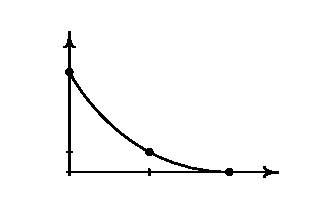
\includegraphics[scale=1.25]{krivka_vyp_t012}\\
   % translate x=-9 y=147 scale 0.30
   \putbox{0.06in}{1.34in}{1.20}{$g(t)$}%
   \putbox{2.11in}{0.09in}{1.20}{$t$}%
   \putbox{1.69in}{0.09in}{1.20}{$t_2$}%
   \putbox{1.02in}{0.09in}{1.20}{$t_1$}%
   \putbox{0.36in}{0.09in}{1.20}{$t_0$}%
   \putbox{0.15in}{0.21in}{1.20}{$G_2$}%
   \putbox{0.15in}{0.38in}{1.20}{$G_1$}%
   \putbox{0.15in}{1.04in}{1.20}{$G_0$}%
   } % close 'parbox'
   } % close 'scalebox'
   \vspace{-\baselineskip} % this is not necessary, but looks better

	\caption{príklad krivky pre vypínací dej}
	\label{fig:krivka_vyp_t012}
\end{figure}


\subsection{Parabola s \uv{nastaviteľným} exponentom}
Hĺbka priehybu parabolickej krivky je daná veľkosťou exponentu. Túto skutočnosť možno využiť k preloženiu analytickej krivky predpokladaného tvaru zmeranými bodmi. Parabola vo všeobecnom tvare $f(t)=a(t+b)^\alpha$ je jednoznačne určená tromi parametrami. Parameter $\alpha$ môže byť párny, nepárny, ako aj neceločíselný (v tom prípade je krivka naznačená na Obr. \ref{fig:patocka_fxfmxfmxpb} vľavo nesymetrická).
\begin{figure}[ht!]
	\centering
	% XCircuit output "skola/5zs/sempr/latex/obr/krivky_patocka_fxfmxfmxpb.tex" for LaTeX input from skola/5zs/sempr/latex/obr/krivky_patocka_fxfmxfmxpb.ps
\def\putbox#1#2#3#4{\makebox[0in][l]{\makebox[#1][l]{}\raisebox{\baselineskip}[0in][0in]{\raisebox{#2}[0in][0in]{\scalebox{#3}{#4}}}}}
\def\rightbox#1{\makebox[0in][r]{#1}}
\def\centbox#1{\makebox[0in]{#1}}
\def\topbox#1{\raisebox{-0.60\baselineskip}[0in][0in]{#1}}
\def\midbox#1{\raisebox{-0.20\baselineskip}[0in][0in]{#1}}
   \scalebox{0.8}{
   \normalsize
   \parbox{5.48438in}{
   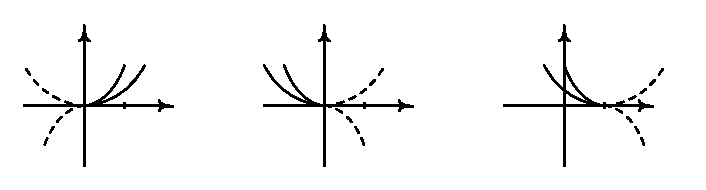
\includegraphics[scale=1.25]{krivky_patocka_fxfmxfmxpb}\\
   % translate x=591 y=207 scale 0.30
   \putbox{0.65in}{1.06in}{1.20}{$f(x)$}%
   \putbox{1.19in}{0.40in}{1.20}{$x$}%
   \putbox{0.86in}{0.40in}{1.20}{$b$}%
   \putbox{2.65in}{1.06in}{1.20}{$f(-x)$}%
   \putbox{3.19in}{0.40in}{1.20}{$x$}%
   \putbox{2.86in}{0.40in}{1.20}{$b$}%
   \putbox{4.65in}{1.06in}{1.20}{$f(-x+b)$}%
   \putbox{5.19in}{0.40in}{1.20}{$x$}%
   \putbox{4.86in}{0.40in}{1.20}{$b$}%
   } % close 'parbox'
   } % close 'scalebox'
   \vspace{-\baselineskip} % this is not necessary, but looks better

	%\caption{K určeniu znamienok vo vzťahu (\ref{eq:})}
	\caption{Operácie so všeobecnou funkciou $f(x)$.}
	\label{fig:patocka_fxfmxfmxpb}
\end{figure}

Úvahou graficky naznačenou na Obr. \ref{fig:patocka_fxfmxfmxpb} možno odvodiť výraz pre vypínací dej:
\begin{equation}
	g_{CE}(t) = 
	\left\{
	\begin{array}{l l}
		G_{CE,sat};	& t<t_0 \\
		G_{CE,sat} \left( 1 - \frac{t-t_0}{t_{off}} \right)^\alpha;	& t_0 \leq t \leq t_0+t_{off} \\
		0;		& t > t_0+t_{off}
	\end{array}
	\right.
	\label{eq:gCE_patocka_valsa}
\end{equation}
kde $t_0$ je okamih počiatku vypínacieho deja, $t_{off}$ je celková vypínacia doba deja, $G_{CE,sat} = \frac{I_L}{U_{CE,sat}}$.
Tento vzťah bol odvodený v \cite{valsa-patocka-petru}. Pre výpočet parametru $\alpha$ autori uvádzajú vzťah:
\begin{equation}
	\alpha = \frac{\ln\left( U_d / U_{CE,sat} \right)}{\ln\left( t_{off} / t_f \right)}
	\label{eq:patocka_alpha}
\end{equation}

Pre zapínací dej autori odvodili obdobný vzťah.

Táto aproximácia sa osvedčila v dobe citovaného článku pre vtedajšie bipolárne tranzistory pre svoju jednoduchosť (pri $t_0 = 0$ a $G_{off} = 0$ stačí zadávať tri čísla z merania) a dobrý súlad so skutočným priebehom $g_{CE} = \frac{i_{C}}{u_{CE}}$. 

Pre súčasné unipolárne a hlavne IGBT tranzistory, kde sa kombinuje rýchle zavretie MOSFET štruktúry s následným pomalším vypínaním štruktúry PNP, s typickým \uv{chvostom} v priebehu $i_C$ môže byť tento jednoduchý model tvarovo nepostačujúci.


\subsection{Interpolačný polynóm}
Väčšiu tvarovú flexibilitu a zároveň jeden funkčný predpis na celom intervale $(t_0, t_2)$ poskytuje interpolácia polynómu zmeranými bodmi.\\
Jednoduchý algoritmus dosadzovania hodnôt priamo z predpisu tabuľkou (\ref{eq:tab_predpis_t012}) poskytuje Lagrangeov polynóm $n$-tého rádu v tvare:
\begin{equation}
	P_n(t) = \sum_{i=0}^n G_i \cdot l_i(t); 
	\;\;\;\;\;\;\;\;\;\;\;\;\;\;\;\;
	l_i(t) = \prod_{j=0,1,\ldots,n; j\neq i} \frac{t - t_j}{t_i - tj}
	\label{eq:Lagrange_vseobec}
\end{equation}
teda napr. pre 3 body z predpisu (\ref{eq:tab_predpis_t012}):
\begin{equation}
	P_2(t) = G_0 \cdot \frac{(t-t_1)(t-t_2)}{(t_0-t_1)(t_0-t_2)} + G_1 \cdot \frac{(t-t_0)(t-t_2)}{(t_1-t_0)(t_1-t_2)} + G_2 \cdot \frac{(t-t_0)(t-t_1)}{(t_2-t_0)(t_2-t_1)}
	\label{Lagrange_z_tabulky}
\end{equation}

\begin{figure}[ht!]
	\centering
	% XCircuit output "Lagrange_vseobec.tex" for LaTeX input from Lagrange_vseobec.ps
\def\putbox#1#2#3#4{\makebox[0in][l]{\makebox[#1][l]{}\raisebox{\baselineskip}[0in][0in]{\raisebox{#2}[0in][0in]{\scalebox{#3}{#4}}}}}
\def\rightbox#1{\makebox[0in][r]{#1}}
\def\centbox#1{\makebox[0in]{#1}}
\def\topbox#1{\raisebox{-0.60\baselineskip}[0in][0in]{#1}}
\def\midbox#1{\raisebox{-0.20\baselineskip}[0in][0in]{#1}}
   \scalebox{0.8}{
   \normalsize
   \parbox{3.02083in}{
   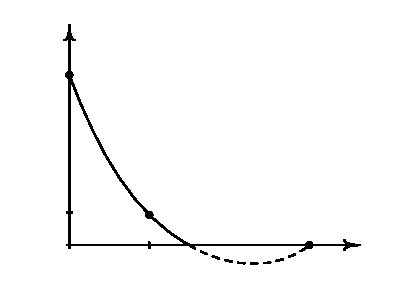
\includegraphics[scale=1.25]{Lagrange_vseobec}\\
   % translate x=-9 y=147 scale 0.30
   \putbox{0.06in}{1.92in}{1.20}{$g(t)$}%
   \putbox{2.77in}{0.09in}{1.20}{$t$}%
   \putbox{2.44in}{0.09in}{1.20}{$t_2$}%
   \putbox{1.02in}{0.09in}{1.20}{$t_1$}%
   \putbox{0.36in}{0.09in}{1.20}{$t_0$}%
   \putbox{0.15in}{0.21in}{1.20}{$G_2$}%
   \putbox{0.15in}{0.48in}{1.20}{$G_1$}%
   \putbox{0.15in}{1.63in}{1.20}{$G_0$}%
   } % close 'parbox'
   } % close 'scalebox'
   \vspace{-\baselineskip} % this is not necessary, but looks better

	\caption{Polynóm 2. stupňa (preložený tromi bodmi).}
	\label{fig:Lagrange_vseobec}
\end{figure}

Primárnym účelom Lagrangeovho polynómu je preloženie krivky danými bodmi; nie je vylúčená situácia znázornená na Obr. \ref{fig:Lagrange_vseobec} (je naopak pomerne pravdepodobná), teda vznik intervalov s kladnou deriváciou (sklonom) či dokonca úsek so zápornou vodivosťou. Takáto situácia je nie len fyzikálne nezmyselná, ale tiež predstavuje výpočtové problémy v prípade zaradenia vodivosti do numericky riešeného obvodu.

Jednoduchý polynóm preložený cez 3 body preto nie je príliš sľubnou aproximáciou.


\subsection{Krivky definované na dvoch subintervaloch s hraničnými podmienkami}

Krivku možno tiež definovať zvlášť na jednotlivých intervaloch medzi danými bodmi:
\begin{equation}
	g_{CE}(t) = 
	\left\{
	\begin{array}{l l}
		G_0;	& t<t_0 \\
		g_1(t);	& t_0 \leq t < t_1 \\
		g_2(t);	& t_1 \leq t < t_2 \\
		G_2;		& t \geq t_2
	\end{array}
	\right.
	\label{eq:krivka_subintervaly_gong1g2goff}
\end{equation}

Požadované vlastnosti výslednej krivky definujú hraničné podmienky pre jednotlivé krivky
.

Pre jednoduchosť definujme na podintervaloch parabolické krivky druhého rádu v názornom tvare pre vynášanie do grafu:

\begin{subequations} 
	\label{eq:def_g1_g2_klm_obe}
	\begin{align}
		g_1(t) = k_1 (l_1 - t)^2 + m_1	%\label{eq:def_g1_g2_klm_1}
		\\
		g_2(t) = k_2 (l_2 - t)^2 + m_2	%\label{eq:def_g1_g2_klm_2}
	\end{align}
\end{subequations}

Roznásobením zátvorky dostaneme po substitúciach
\begin{subequations} 
	\label{eq:subst_klm2abc}
	\begin{align}
		a_i = k_i\\
		b_i = -2 k_i l_i\\
		c_i = k_i l_i^2 + m_i
	\end{align}
\end{subequations}
tvar rovníc zapisovateľný do matice, tj, pre neznáme $a_i$, $b_i$, $c_i$ sa jedná o lineárne rovnice:
\begin{subequations} 
	\label{eq:def_g1_g2_abc_obe}
	\begin{align}
		g_1(t) = a_1 t^2 + b_1 t + c_1	\label{eq:def_g1_g2_abc_1}\\
		g_2(t) = a_2 t^2 + b_2 t + c_2	\label{eq:def_g1_g2_abc_2}
	\end{align}
\end{subequations}

Vo funkciách (\ref{eq:def_g1_g2_abc_obe}) vystupuje 6 neznámych. Na ich vyriešenie je preto nutné zostaviť systém 6 rovníc takých, aby výsledné funkcie spĺňali požadované vlastnosti.\\
Zaveďme teda tieto predpoklady (okrajové podmienky):
\begin{myass}
	$g_1(t_0) = G_0$
	\label{myass:1}
\end{myass}
\begin{myass}
	$g_1(t_1) = G_1$
	\label{myass:2}
\end{myass}
\begin{myass}
	$g_2(t_1) = G_1$
	\label{myass:3}
\end{myass}
\begin{myass}
	$g_2(t_2) = G_2$
	\label{myass:4}
\end{myass}
\begin{myass}
	$g_1'(t_1) = g_2'(t_1)$ \ldots hladkosť krivky v bode $t=t_1$
	\label{myass:5}
\end{myass}
\begin{myass}
	$g_2'(t_2)=0$ \ldots hladkosť v bode $t=t_2$
	\label{myass:6}
\end{myass}
\vspace{12pt}

Derivovaním (\ref{eq:def_g1_g2_klm_obe}) resp. (\ref{eq:def_g1_g2_abc_obe}) podľa času dostávame:

\begin{subequations} 
	\label{eq:def_g1_g2_deriv_klm_obe}
	\begin{align}
		g_1'(t) = -2 k_1 (l_1 -t) 	\label{eq:def_g1_g2_deriv_klm_1} \\
		g_2'(t) = -2 k_2 (l_2 -t) 	\label{eq:def_g1_g2_deriv_klm_2}
	\end{align}
\end{subequations}

\begin{subequations} 
	\label{eq:def_g1_g2_deriv_abc_obe}
	\begin{align}
		g_1'(t) = 2 a_1 t + b_1 	\label{eq:def_g1_g2_deriv_abc_1} \\
		g_2'(t) = 2 a_2 t + b_2 	\label{eq:def_g1_g2_deriv_abc_2}
	\end{align}
\end{subequations}

Dosadením predpokladov (\ref{myass:1}) až (\ref{myass:6}) do (\ref{eq:def_g1_g2_abc_obe}), (\ref{eq:def_g1_g2_deriv_abc_obe}) získame jednoznačne riešiteľnú sústavu v maticovom tvare zapísanú ako:

\begin{equation}
	\underbrace
	{
		\left( 
		\begin{array}{c c c c c c}
			t_0^2& t_0& 1& 0& 0& 0\\
			t_1^2 &t_1 &1 &0 & 0& 0 \\
			0& 0& 0& t_1^2& t_1& 1 \\
			0& 0& 0& t_2^2& t_2& 1 \\
			2t_1& 1& 0& -2t_1& -1& 0 \\
			0& 0& 0& 2t_1& 1& 0
		\end{array}
		\right)
	}_{[M]}
	\cdot
	\underbrace
	{
		\left(
		\begin{array}{c}
			a_1 \\
			b_1 \\
			c_1 \\
			a_2 \\
			b_2 \\
			c_2
		\end{array}
		\right)
	}_{\mathbf{X}}
	=
	\underbrace
	{
		\left( 
		\begin{array}{c}
			G_0 \\
			G_1 \\
			G_1 \\
			G_2 \\
			0 \\
			0
		\end{array}
		\right)
	}_{\mathbf{V}}
	\label{eq:krivka_matica_sustavy}
\end{equation}

kde $[M]$ je matica sústavy, ktorej všetky prvky sú známe (z predpisu (\ref{eq:tab_predpis_t012})), $\mathbf{X}$ je vektor neznámych hľadaných parametrov a $\mathbf{V}$ je známy vektor výsledkov rovníc.

Riešením sústavy je:
\begin{equation}
	\mathbf{X} = [M]^{-1} \cdot \mathbf{V}
	\label{eq:krivka_riesenie_abc}
\end{equation}

V programe \textit{Octave} (alebo \textsc{Matlab}) možno na riešenie takejto sústavy použiť jeden príkaz bez nutnosti vyčísľovania inverznej matice:
\begin{verbatim}
X = M \ V
\end{verbatim}

Program na obvodové simulácie \textsc{Spice} neponúka príliš široké matematické možnosti, čo zvlášť platí pre pôvodnú verziu \textsc{Spice 3} z univerzity v Berkeley, ktorý možno považovať za štandard a preto je jedným z cieľov tejto práce model kompatibilný práve so \textsc{Spice 3}.

Je preto vhodné vyjadriť jednotlivé koeficienty funkcii $g_1$, $g_2$ analyticky. Na tento účel je vhodnejší tvar rovníc (\ref{eq:def_g1_g2_klm_obe}), (\ref{eq:def_g1_g2_deriv_klm_obe}).
Postupným dosadzovaním predpokladov (\ref{myass:6}), (\ref{myass:4}), (\ref{myass:3}) do príslušných rovníc sú vyjadrené koeficienty $l_2$, $m_2$, $k_2$.
Následným dosadením predpokladov (\ref{myass:1}), (\ref{myass:2}), (\ref{myass:5}) sú vyjadrené zvyšné koeficienty $l_1$, $m_1$, $k_1$:

\begin{equation}
	\begin{array}{r l}
		k_2& = \frac{G_1-G_2}{(t_2-t_1)^2} \\
		l_2& = t2 \\
		m_2& = G_2 \\
		l_1& = \frac{(t_1-t_0)^2 (G_1 - G_2) - t_1(t_2-t_1)}{2(t_1-t_0)(G_1-G_2) - (t_2-t_1)(G_0-G_1)} \\
		k_1& = \frac{G_1-G_2}{(t_2-t_1)(l_1-t_1)} \\
		m_1& = G_0 - k1(l_1 - t_0)^2
	\end{array}
	\label{eq:krivka_riesenie_klm}
\end{equation}

Sústavu podobnú sústave (\ref{eq:krivka_matica_sustavy} je jednoduchým spôsobom možné definovať a riešiť numericky pomocou výpočtových programov aj pre zapínací dej a takisto pre viacero subintervalov. V prípade potreby je možné definovať vlastnosti výslednej krivky inými okrajovými podmienkami pre jednotlivé funkcie.

Poznamenajme, že $G_1 = G_{CE,sat}=\frac{I_L}{U_{CE,sat}}$, $G_2 = G_{off} \approx 0$, $t_2 = t_0+t_{off}$ a $t_1$ a $G_1$ závisí na konkrétnej podobe (\ref{eq:tab_predpis_t012}). Koeficienty $a_i$, $b_i$, $c_i$ sú ekvivalentné s koeficientami $k_i$, $l_i$, $m_i$ s prepočítavacím vzťahom cez substitúcie (\ref{eq:subst_klm2abc}).



Metóda dvoch funkcií na subintervaloch je použiteľná aj pre \uv{menej hladké} priebehy, ako je napr. \uv{chvost} vypínaného prúdu IGBT tranzistorom. Na Obr. \ref{fig:tail} je vyobrazený takýto prípad (horšie modelovateľný pomocou jednoduchej paraboly)

\begin{figure}
	\centering
	% GNUPLOT: LaTeX picture with Postscript
\begingroup
  \makeatletter
  \providecommand\color[2][]{%
    \GenericError{(gnuplot) \space\space\space\@spaces}{%
      Package color not loaded in conjunction with
      terminal option `colourtext'%
    }{See the gnuplot documentation for explanation.%
    }{Either use 'blacktext' in gnuplot or load the package
      color.sty in LaTeX.}%
    \renewcommand\color[2][]{}%
  }%
  \providecommand\includegraphics[2][]{%
    \GenericError{(gnuplot) \space\space\space\@spaces}{%
      Package graphicx or graphics not loaded%
    }{See the gnuplot documentation for explanation.%
    }{The gnuplot epslatex terminal needs graphicx.sty or graphics.sty.}%
    \renewcommand\includegraphics[2][]{}%
  }%
  \providecommand\rotatebox[2]{#2}%
  \@ifundefined{ifGPcolor}{%
    \newif\ifGPcolor
    \GPcolorfalse
  }{}%
  \@ifundefined{ifGPblacktext}{%
    \newif\ifGPblacktext
    \GPblacktexttrue
  }{}%
  % define a \g@addto@macro without @ in the name:
  \let\gplgaddtomacro\g@addto@macro
  % define empty templates for all commands taking text:
  \gdef\gplbacktext{}%
  \gdef\gplfronttext{}%
  \makeatother
  \ifGPblacktext
    % no textcolor at all
    \def\colorrgb#1{}%
    \def\colorgray#1{}%
  \else
    % gray or color?
    \ifGPcolor
      \def\colorrgb#1{\color[rgb]{#1}}%
      \def\colorgray#1{\color[gray]{#1}}%
      \expandafter\def\csname LTw\endcsname{\color{white}}%
      \expandafter\def\csname LTb\endcsname{\color{black}}%
      \expandafter\def\csname LTa\endcsname{\color{black}}%
      \expandafter\def\csname LT0\endcsname{\color[rgb]{1,0,0}}%
      \expandafter\def\csname LT1\endcsname{\color[rgb]{0,1,0}}%
      \expandafter\def\csname LT2\endcsname{\color[rgb]{0,0,1}}%
      \expandafter\def\csname LT3\endcsname{\color[rgb]{1,0,1}}%
      \expandafter\def\csname LT4\endcsname{\color[rgb]{0,1,1}}%
      \expandafter\def\csname LT5\endcsname{\color[rgb]{1,1,0}}%
      \expandafter\def\csname LT6\endcsname{\color[rgb]{0,0,0}}%
      \expandafter\def\csname LT7\endcsname{\color[rgb]{1,0.3,0}}%
      \expandafter\def\csname LT8\endcsname{\color[rgb]{0.5,0.5,0.5}}%
    \else
      % gray
      \def\colorrgb#1{\color{black}}%
      \def\colorgray#1{\color[gray]{#1}}%
      \expandafter\def\csname LTw\endcsname{\color{white}}%
      \expandafter\def\csname LTb\endcsname{\color{black}}%
      \expandafter\def\csname LTa\endcsname{\color{black}}%
      \expandafter\def\csname LT0\endcsname{\color{black}}%
      \expandafter\def\csname LT1\endcsname{\color{black}}%
      \expandafter\def\csname LT2\endcsname{\color{black}}%
      \expandafter\def\csname LT3\endcsname{\color{black}}%
      \expandafter\def\csname LT4\endcsname{\color{black}}%
      \expandafter\def\csname LT5\endcsname{\color{black}}%
      \expandafter\def\csname LT6\endcsname{\color{black}}%
      \expandafter\def\csname LT7\endcsname{\color{black}}%
      \expandafter\def\csname LT8\endcsname{\color{black}}%
    \fi
  \fi
  \setlength{\unitlength}{0.0500bp}%
  \begin{picture}(4320.00,4320.00)%
    \gplgaddtomacro\gplbacktext{%
      \csname LTb\endcsname%
      \put(176,2379){\rotatebox{-270}{\makebox(0,0){\strut{}$g_{CE}$, $v_{CE}$, $i_C$}}}%
      \put(2159,440){\makebox(0,0){\strut{}ČAS}}%
    }%
    \gplgaddtomacro\gplfronttext{%
    }%
    \gplgaddtomacro\gplbacktext{%
      \csname LTb\endcsname%
      \put(396,2379){\rotatebox{-270}{\makebox(0,0){\strut{}}}}%
      \put(2159,594){\makebox(0,0){\strut{}}}%
    }%
    \gplgaddtomacro\gplfronttext{%
    }%
    \gplgaddtomacro\gplbacktext{%
      \csname LTb\endcsname%
      \put(396,2379){\rotatebox{-270}{\makebox(0,0){\strut{}}}}%
      \put(2159,594){\makebox(0,0){\strut{}}}%
    }%
    \gplgaddtomacro\gplfronttext{%
    }%
    \gplbacktext
    \put(0,0){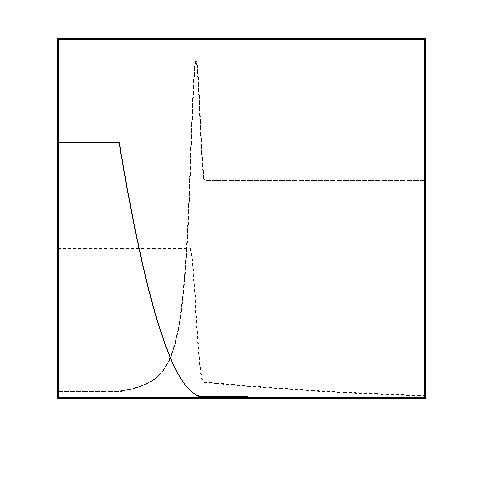
\includegraphics{./tail}}%
    \gplfronttext
  \end{picture}%
\endgroup

	\caption{Možnosti modelu definovaného dvomi krivkami na podintervaloch.}
	\label{fig:tail}
\end{figure}

